\documentclass{mimosis}

\usepackage{metalogo}

%%%%%%%%%%%%%%%%%%%%%%%%%%%%%%%%%%%%%%%%%%%%%%%%%%%%%%%%%%%%%%%%%%%%%%%%
% Some of my favourite personal adjustments
%%%%%%%%%%%%%%%%%%%%%%%%%%%%%%%%%%%%%%%%%%%%%%%%%%%%%%%%%%%%%%%%%%%%%%%%
%
% These are the adjustments that I consider necessary for typesetting
% a nice thesis. However, they are *not* included in the template, as
% I do not want to force you to use them.

% This ensures that I am able to typeset bold font in table while still aligning the numbers
% correctly.
\usepackage{etoolbox}

\usepackage[binary-units=true]{siunitx}
\DeclareSIUnit\px{px}

\sisetup{%
  detect-all           = true,
  detect-family        = true,
  detect-mode          = true,
  detect-shape         = true,
  detect-weight        = true,
  detect-inline-weight = math,
}

%%%%%%%%%%%%%%%%%%%%%%%%%%%%%%%%%%%%%%%%%%%%%%%%%%%%%%%%%%%%%%%%%%%%%%%%
% Hyperlinks & bookmarks
%%%%%%%%%%%%%%%%%%%%%%%%%%%%%%%%%%%%%%%%%%%%%%%%%%%%%%%%%%%%%%%%%%%%%%%%

\usepackage[%
  colorlinks = true,
  citecolor  = RoyalBlue,
  linkcolor  = RoyalBlue,
  urlcolor   = RoyalBlue,
  unicode,
  ]{hyperref}

\usepackage{bookmark}

%%%%%%%%%%%%%%%%%%%%%%%%%%%%%%%%%%%%%%%%%%%%%%%%%%%%%%%%%%%%%%%%%%%%%%%%
% Bibliography
%%%%%%%%%%%%%%%%%%%%%%%%%%%%%%%%%%%%%%%%%%%%%%%%%%%%%%%%%%%%%%%%%%%%%%%%
%
% I like the bibliography to be extremely plain, showing only a numeric
% identifier and citing everything in simple brackets. The first names,
% if present, will be initialized. DOIs and URLs will be preserved.

\usepackage[%
  autocite     = plain,
  backend      = bibtex,
  doi          = true,
  url          = true,
  giveninits   = true,
  hyperref     = true,
  maxbibnames  = 99,
  maxcitenames = 99,
  sortcites    = true,
  style        = numeric,
  ]{biblatex}

%%%%%%%%%%%%%%%%%%%%%%%%%%%%%%%%%%%%%%%%%%%%%%%%%%%%%%%%%%%%%%%%%%%%%%%%
% Tables
%%%%%%%%%%%%%%%%%%%%%%%%%%%%%%%%%%%%%%%%%%%%%%%%%%%%%%%%%%%%%%%%%%%%%%%%
%
% DEFINED BY RUI - NOT IN THE TEMPLATE

\usepackage{tabulary}
\usepackage[export]{adjustbox} % To put borders around some figures

%\input{bibliography-mimosis}
\addbibresource{Thesis.bib}

%%%%%%%%%%%%%%%%%%%%%%%%%%%%%%%%%%%%%%%%%%%%%%%%%%%%%%%%%%%%%%%%%%%%%%%%
% Fonts
%%%%%%%%%%%%%%%%%%%%%%%%%%%%%%%%%%%%%%%%%%%%%%%%%%%%%%%%%%%%%%%%%%%%%%%%

\ifxetexorluatex
  \setmainfont{Minion Pro}
\else
  \usepackage[lf]{ebgaramond}
  \usepackage[oldstyle,scale=0.7]{sourcecodepro}
  \singlespacing
\fi

\renewcommand{\th}{\textsuperscript{\textup{th}}\xspace}

%\newacronym[description={Principal component analysis}]{PCA}{PCA}{principal component analysis}
\newacronym                                            {sdn}{SDN}{Software-defined networking}
\newacronym                                            {api}{API}{Application Programming Interface}
\newacronym                                            {vpcs}{VPCS}{Simple Virtual PC Simulator}
\newacronym                                            {dhcp}{DHCP}{Dynamic Host Configuration Protocol}
\newacronym                                            {rest}{REST}{Representational state transfer} % TODO put it the glossary
\newacronym                                            {nic}{NIC}{network interface controller} % TODO put it the glossary
\newacronym                                            {mtu}{MTU}{maximum transmission unit} % TODO put it the glossary
\newacronym                                            {nat}{NAT}{network address translation}

\newglossaryentry{LaTeX}{%
  name        = {\LaTeX},
  description = {A document preparation system},
  sort        = {LaTeX},
}

\newglossaryentry{Real numbers}{%
  name        = {$\real$},
  description = {The set of real numbers},
  sort        = {Real numbers},
}

% TODO Add entry for REST
% TODO Add entry for WebSockets

\makeindex
\makeglossaries

%%%%%%%%%%%%%%%%%%%%%%%%%%%%%%%%%%%%%%%%%%%%%%%%%%%%%%%%%%%%%%%%%%%%%%%%
% Incipit
%%%%%%%%%%%%%%%%%%%%%%%%%%%%%%%%%%%%%%%%%%%%%%%%%%%%%%%%%%%%%%%%%%%%%%%%

%%%%%%%%%%%%%%%%%%%%%%%%%%%%%%%%%%%%%%%%%%%%%%%%%%%%%%%%%%%%%%%%%%%%%%%%
% Rui's LaTeX and/or editor hacks and notes go here.
% e.g. useful regex to search for in the file.
% Things we want to look for:
% Comments starting with the "TODO" string
% Lines (in the text file) that contain more than two sentence.
% Take into account that some sentences end in doube-quotes
% (with the perid . before it)
%
% TODO Use the oxford comma?
% TODO see how dates are written in English across the whole document
% TODO check if there are i.e. with a "comma" after it
% TODO check how many text between parenthesis and m-dashes is there
% TODO check for double-quote american errors, i.e. commas out of "",
% TODO check for <CAPS LOCK STUFF INSIDE ST/GT SIGNS>
%%%%%%%%%%%%%%%%%%%%%%%%%%%%%%%%%%%%%%%%%%%%%%%%%%%%%%%%%%%%%%%%%%%%%%%%

\title{Usage of network emulators for the benefit of teaching and learning}
%\subtitle{A minimal, modern \LaTeX{} package for typesetting your thesis}
\author{Rui Miguel Carrilho Carvalho}

\begin{document}

\frontmatter
  % !TEX root = ../Thesis.tex
\begin{titlepage}
  \vspace*{5cm}
  \makeatletter
  \begin{center}
    \begin{Huge}
      \@title
    \end{Huge}\\[0.1cm]
    %
    % \begin{Large}
    %   \@subtitle
    % \end{Large}\\
    %
    % \emph{by}\\
    \@author
    %
    \vfill
    A document submitted in partial fulfillment
    of the requirements for the degree of\\
    \emph{Technical Report}\\
    at\\
    \textsc{Miskatonic University}
  \end{center}
  \makeatother
\end{titlepage}

\newpage
\null
\thispagestyle{empty}
\newpage

  % !TEX root = ../Thesis.tex
% !TEX spellcheck = en-US

\begin{center}
  \textsc{Abstract}
\end{center}
%
\noindent
%
Scientific documents often use \LaTeX{} for typesetting. While numerous
packages and templates exist, it makes sense to create a new one. Just
because.


  \tableofcontents

\mainmatter

  % !TEX root = ../Thesis.tex
% !TEX spellcheck = en-US

\chapter{Introduction}
\label{ch:introduction}

This first chapter introduces the challenge of using virtual, fully software-based alternatives to computer network labs in education, with special emphasis on the undergraduate and graduate levels of the university. % TODO should university by capitalized here?
It gives reasons to do so, and provides an overview of the work that has already been done both in development of those kinds of tools and in their current introduction, and study thereof, in existing universities and courses.
Furthermore, it explains the motivation behind the main work performed in the present document, which consists in studying and comparing different existing software solutions for simulating and emulating computer networks and, both theoretically and practically, justifying how each one can or cannot be a got fit for particular use-cases of different courses or subjects inside computer networks studying.

% It also proposes the definitions that, though not universal or unique, help precise differences between those software solutions, namely two main concepts: simulation and emulation. % TODO universal NOR unique?
% Together with the last point, this chapter also explains the reason why this thesis is centered, starting from its title, in ``emulators'' more than on ``simulators''.
% Finally, it gives a very brief overview of the work that has already been done in the field of computer networks simulators and emulators, and, orthogonally, in the replacement of laboratories with (physical) hosts and routers/switches in schools and universities by simulated or emulated (virtual) solutions.

\section{Motivation and problem statement}
\label{sec:motivation}

Teaching of computer networks courses and subjects, to fulfill the desired properties of a ``hands-on approach'' in engineering, one which enables putting in practice the knowledge acquired in the theoretical component of subjects, typically require performing two kinds of exercises: i. on the application layer, using APIs that give access to the OS's network-stack and the host interfaces; and, ii. on ``lower layers'' of the stack, oftentimes using physical labs, rooms equipped with networking gear, like switches and routers. % TODO glossário: APIs; citar referências às ditas "propriedades desejáveis"
The existence of those laboratories is, even today, standard practice in many institutions of higher education. FCT/NOVA, which is not an exception, has a room with routers and switches for performing those practical exercises. % TODO inserir aqui fotografia do laboratório da FCT/NOVA?

Despite its virtues, this method for interacting with switching and routing, its protocols, the impacts of different parameters and node behavior on the behavior of a complex application that relies on the network, raises problems such as the cost and fast obsolescence~\cite{automaticnetconfiggns} of equipments, the demand for individual presence on the laboratory (at least for manipulating physical links and network interfaces) for exercise elaboration, the possible damage due to misuse~\cite{teachinginovation} or simple wear-and-tear, the time and effort to prepare and setup for given exercises, which may ``destroy'' the setup for other exercises, etc. % TODO avoid repeating "exercise" so much here

Aiming to address these problems, not exclusive from further or higher education, common to vocational education on high schools and ``\emph{politécnicos},'' and ``courses'' of the industry itself, of which Cisco's CCNA~\cite{ccna} is a prominent example, or even distance learning, tools for emulating and/or simulating networks and networking equipment have been developed for years. % TODO replace "extending". o "vocational education" veio do linguee
% In particular, emulators, much more powerful, flexible, and easier to use in the past due to the recent improvement in computer resources available, and also software technologies, as will be seen later, can provide real interactions...
These tools can, through the usage of several techniques, surpass some (if not all) of the aforementioned disadvantages.
Critically evaluate whether one or more than one, used in a complementary fashion, of the existing simulators/emulators can live up to that ``promise'' is, in a few words, the goal of this work.

% \subsection{The lab on a laptop}
% \label{subsec:thelabonalaptop}

% A very important question that must be taken into account is that the functional hyper-realism of emulators comes at a cost of a lot of resources.
% One or more machines must run a potentially high number of processes where the code that typically runs inside \textbf{each slice} of the stack for \textbf{each node} of the topologies is executed, in a highly concurrent fashion.
% The performance of the hardware can degrade and the observed behavior of the topology may look very unrealistic compared to ``the real thing,'' as obviously there may be less aggregate computing power

\section{Structure of the thesis}
\label{sec:structure}

% end of chapter
 % Chapter 1
  % !TEX root = ../Thesis.tex
% !TEX spellcheck = en-US

\chapter{Related work}
\label{ch:relatedwork}

\section{Emulation and simulation}
\label{sec:emulationsimulation}

Providing a precise definition, or ``definition framework,'' for distinguishing simulators from emulators and why \emph{emulation} (as opposed to \emph{simulation}) is the focus of this dissertation is paramount.
In the literature, Wikipedia, or common dictionaries, there are contradictory definitions, overlapping concepts, and, in general, a vague distinction between the two is presented~\cite{netsimoremu}. % TODO find and insert citations
That is why, rather than universally establishing what an emulator and a simulator are, it is intended that when, throughout this text, software package $A$ is an emulator and $B$ is a simulator in this or that sense, the reader can know without ambiguity what is meant.

% \begin{figure}
%   \centering
%   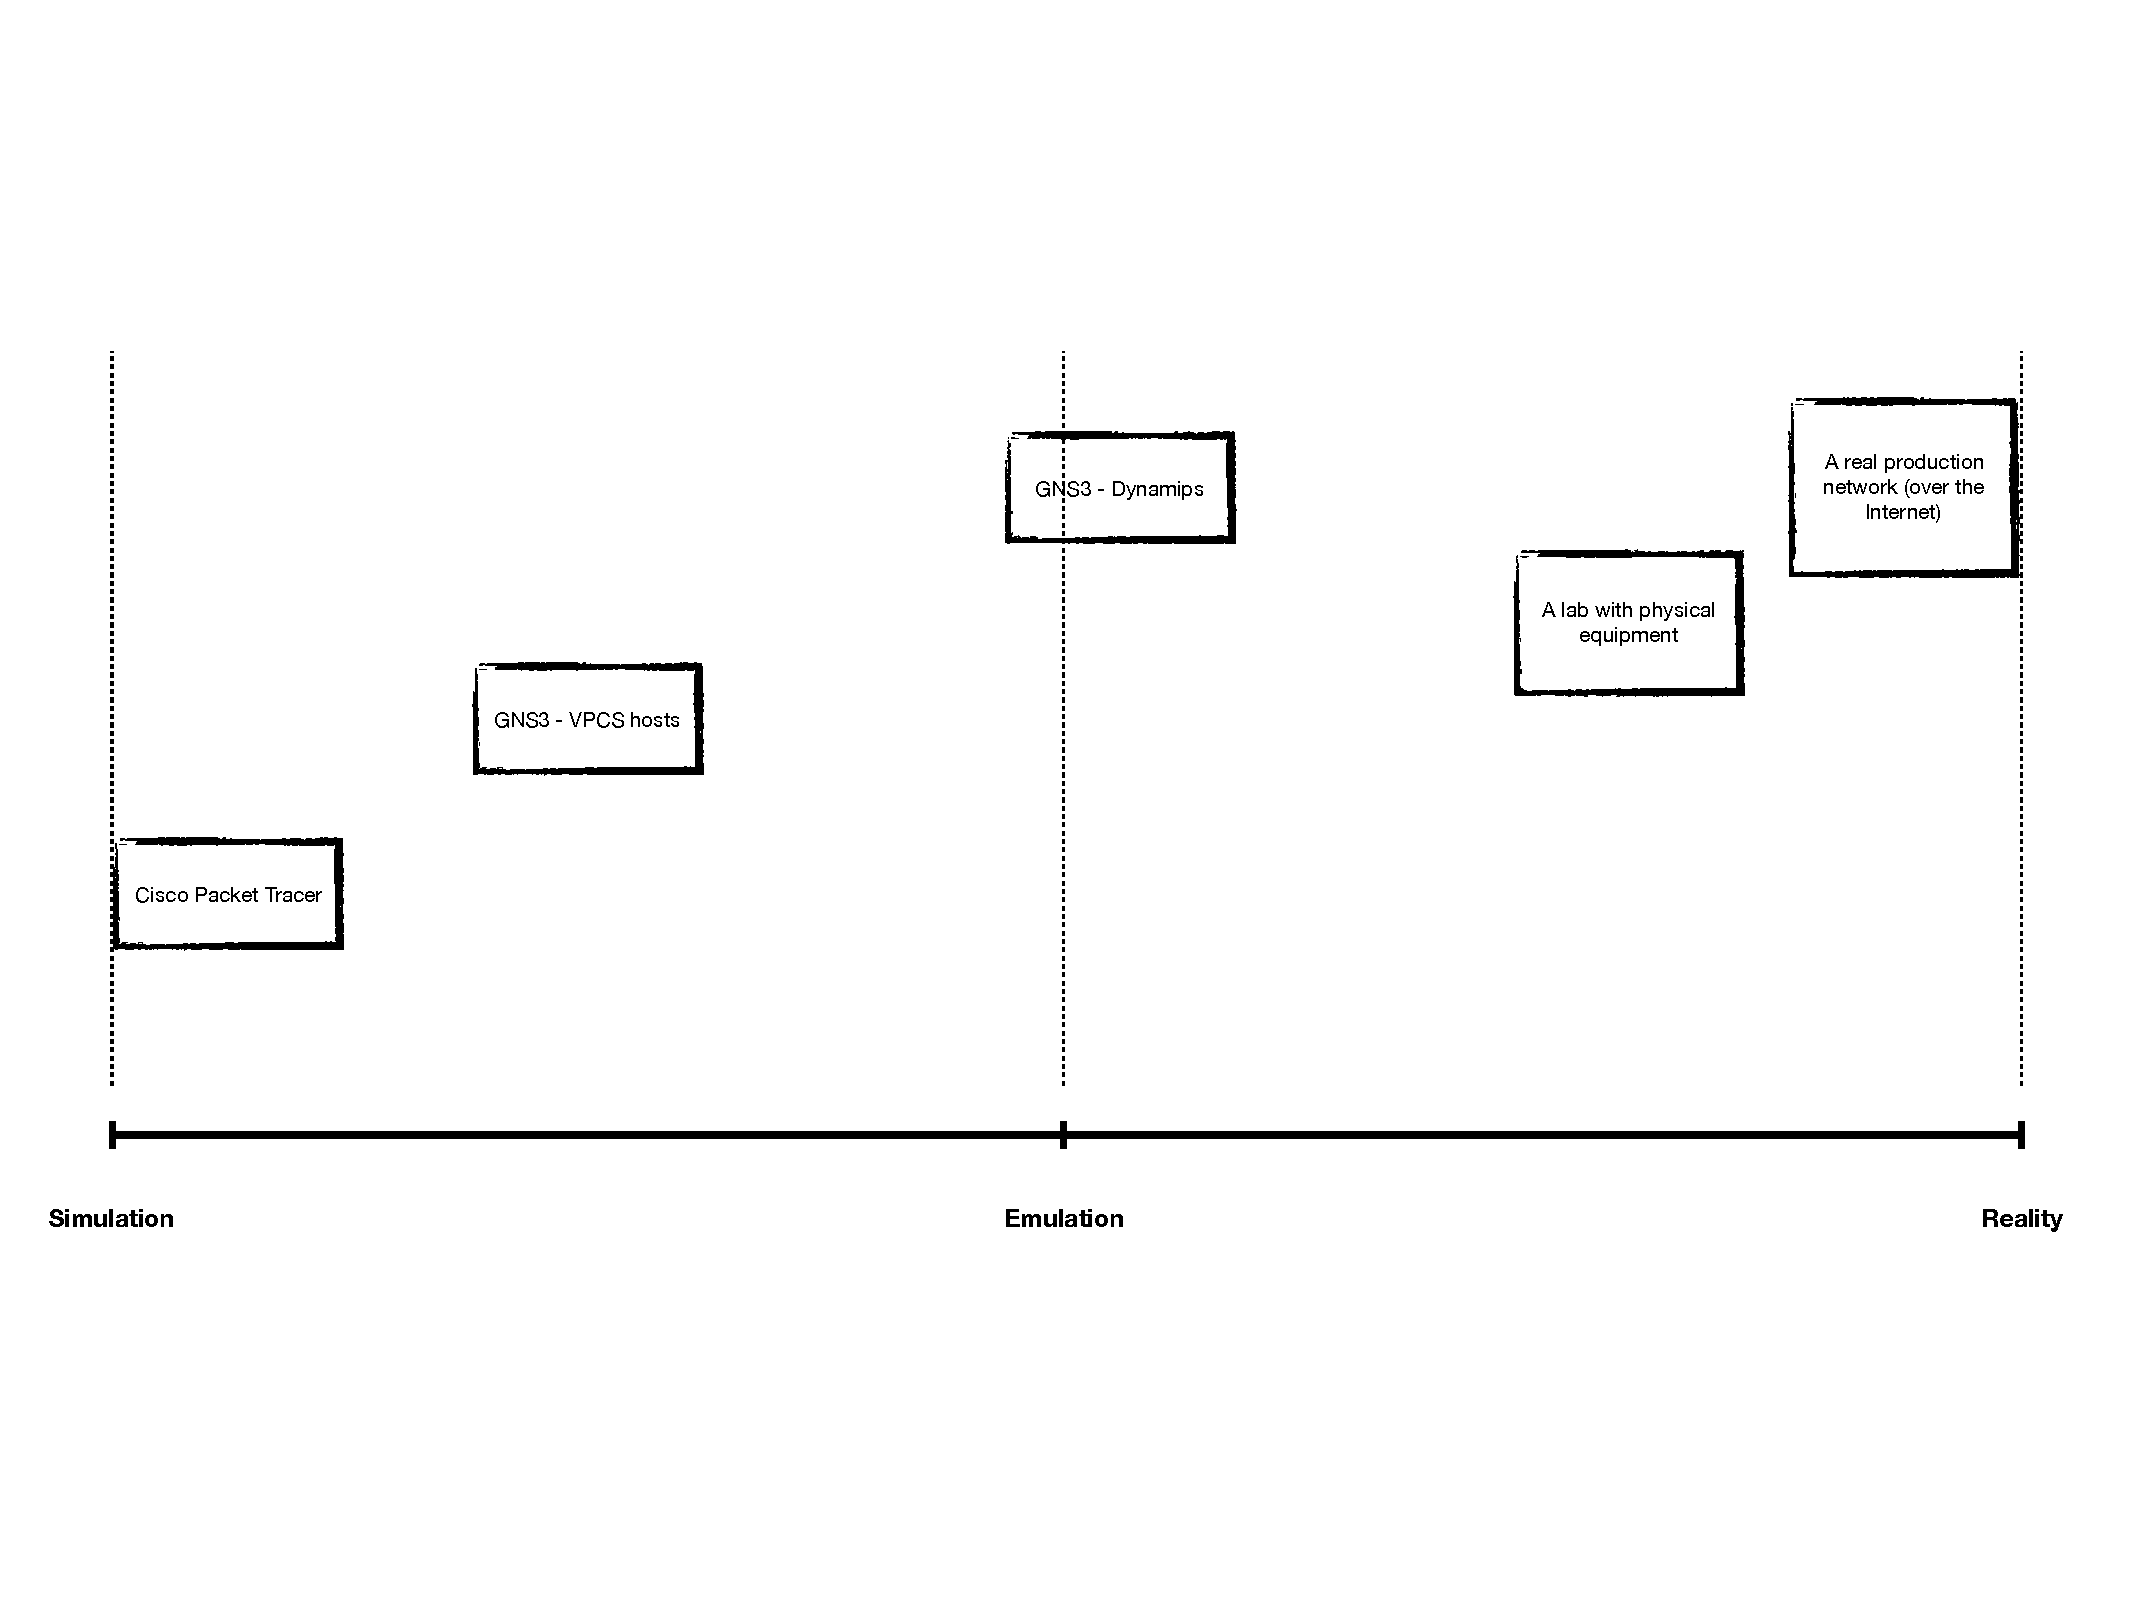
\includegraphics[width=0.8\textwidth]{emulationvsreality}
%   \caption{Simulation vs emulation vs reality}
%   \label{fig:emulationvsreality}
% \end{figure}

Before pointing out the differences between emulators and simulators, it is important to say what both have in common: they are ways of providing students, researches, developers, administrators, or any professional that works with computer networks with an alternative to the real network that is being studied, for convenience and/or cost effectiveness.
However, a lab with network nodes in an education institution is also different from the reality it is trying to model.
%That idea is exposed in the diagram in figure~\ref{fig:emulationvsreality}.

On one end there is reality---in a lab, factors like amount of nodes, physical length of links (and therefore propagation times) can only be \textbf{simulated}, let alone on an solution that is fully software-based, like the emulators described later in this section.
An anecdote like the 500-mile email~\footnote{The case of the 500-mile email~\cite{500mileemail} was an issue described by a systems administrator where e-mails could not be sent to servers further than 500 miles.
The description seemed impossible as e-mail servers (closer) were working, but a hidden configuration---a timeout---rendered a different behavior according to the physical distance between hosts, due to round-trip times.
} could not be reproduced, without simulating an---then---unknown ``flaw,'' in an emulator consisting in virtual machines running the real software and performing the real operations: the cause of the problem was latency.
On the other end there is full simulation, where nothing is real.

In between, complex solutions like GNS3, which is presented in great detail in chapter~\ref{ch:gns3}, can offer a mixture, while being mainly emulators in the sense that it consists in an orchestrated set of processes running the real code, and also allowing to simulate aspects of reality like failures in links and delays.

The reason why emulators are specially interesting and are essentially the motivation (\ref{sec:motivation}) of this work, though, is that giving away the lab room with its switches and cables requires to not lose the flexibility it offers to perform all kind of pedagogical exercises, and ``pure'' simulators do not offer by inherent limitation.

%A network simulator is a computer program (or software package) that implements algorithms corresponding to a \textbf{model} of the reality through software components.
In~\cite{netkit-full}, the article presenting Netkit (a tool studied later in this thesis) and the process that led to its inception, which largely overlaps with the present work, there's an interesting paragraph that explains succinctly the difference between simulation and emulation.
Note that these concepts exist for any kind of \emph{system}, of which any computer system, such as computer networks, are only particular instances:
\begin{displayquote}
Simulation aims at computing the behavior of a network based on an abstract model that usually ignores many functional details (e.g., message formats, the need for configurations, and the presence of command line interfaces).
This approach is suited for massive performance-oriented experiments and usually produces accurate event timing information.
Emulation aims at accurately reproducing the behavior of a real network in all its functional details and is usually achieved by exploiting as much as possible the same software (or an open version of it) that would be used on real devices.
Although considerably less efficient than simulation and usually inadequate to reproduce timings observed in real network systems, this approach is very effective to capture the wide range of functionalities and behaviors of a real network, and we believe it is therefore much more suited for didactics than simulation.
\end{displayquote}
Simulators like ns-3~\cite{ns3} or the OPNET~\cite{introtoopnet} are discrete event simulators~\cite{netsimoremu}.
They enable, through some interface---such as a graphical one---, designing, testing, analyzing, and observing the expected behavior of protocols, nodes, and links according to several parameters. Therefore, it serves as a way to study protocols used across the stack, and possibly even some application layer components can be ``mimicked''.

Even though the usefulness of these tools cannot be questioned, and some like Cisco Packet Tracer~\footnote{\url{https://www.netacad.com/courses/packet-tracer/introduction-packet-tracer}}, also a discrete event simulator~\cite{evaluatingnetsimmethodologicapproach}, are very widely used in the training of professionals in the networks administration and engineering fields~\cite{rolepackettracer}, it is crucial to point out as the distinctive characteristic of simulators, as defined here, the fact that those applications constitute a ``closed'' universe in the sense of only \emph{simulating} events that change the status of internal data structures, but do not implement a real stack of protocols, where every operation that should be performed is, in fact, performed. % TODO this is super "Portuguese in English". Improve

In other words: a network simulator is a black box for the outside, with a set of available inspection and state alteration operations---i.e. that provides the ability to see some aspects of the simulated system and perform some finite set of changes to the simulated environment.
% However, as long as the \emph{implemented} cause-effect behaviors for that set of operations \emph{is coherent} to their real-world counterparts, any kind of ``shortcuts'' inside can be taken.

On the other hand, the definition for an emulator can, therefore, pretty much be inferred from the simulator as its ``complementary.''
Software computer network emulators are solutions that allow, without resorting to the usage of physical equipment (even though sometimes allow for it, if desired) prototyping networks for analysis and study of underlying mechanisms, investigation, and development of new protocols and solutions, etc., thanks to an array of techniques that can span from virtualization and containerization, hardware architecture emulation, and leveraging operating system functionality in multi-process environments.

Unlike the simulators, described earlier, the fact of the traffic being real (at least from a logical standpoint) and that is possible to ``glue'' emulated interfaces with any kind of physical ones detected by the host operating system, offers the possibility of mixing emulated topologies with real topologies, cloud machines, etc.
Besides, since the computational nodes (hosts in the emulated topologies) are in, fact, ``generic'' hosts (nowadays, usually VMs or containers), running real software, the limit in terms of what it is possible to configure, parameterize, implement, or test, for any stack level (from the link to the application layer) is virtually nonexistent.

% \section{Notable simulators}
% \label{sec:notablsimulators}

% Packet Tracer, Boson NetSim, ns-3...

% \section{Notable emulators}
% \label{sec:notablemulators}

% \subsection{GNS3}
% \label{subsec:relworkgns3}

% \subsubsection{Usage of GNS3 in education}
% \label{subsubsec:relgns3usageedu}

% There is already some published work about using GNS3 in education institutions.
% Usually, though, the experiments and comparisons are made against other ``graphical simulators''---instead of emulators---, since those are the software tools that, from a high-level perspective are equivalent, even if the functional possibilities and implementations are completely different, if not opposite.

% A brief comparison with Boson NetSim and Packet Tracer, two graphical simulators, is presented in~\cite{virtlabgnsvmware}, where the authors explain a way to use VMware Workstation VMs on a desktop to ``emulate'' end hosts on GNS3's virtual topologies, and using applications on those VMs which communicate with each other over the emulated links.

% In~\cite{automaticnetconfiggns}, the authors, two Professors from the Polytechnic Institute of Leiria, Portugal, dive into ways to automate GNS3 topology configurations, which, as will be seen in chapter~\ref{ch:gns3}, can be a major issue. % TODO

% The usefulness for distance learning is also explored, for example, in~\cite{networkvirtwithgns}.

% \subsection{Kathara}
% \label{subsec:relworkkathara}

% \subsection{CORE}
% \label{subsec:relworkcore}

% \subsection{Mininet}
% \label{subsec:relworkmininet}

% \section{Usage of simulators and emulators in teaching}
% \label{sec:simemulusage}

% end of chapter
 % Chapter 2
  % !TEX root = ../Thesis.tex
% !TEX spellcheck = en-US

\chapter{GNS3}
\label{ch:gns3}

GNS3, whose original name was ``Graphical Network Simulator-3,'' is a software project, comprising several distinct components and, despite the ``simulator'' in its name, \emph{as a whole}, it falls under the category of emulators (cf.~\ref{sec:emulationsimulation}): its operation runs real code accross all the layers of the stack. % TODO try to (either with a source, or speculating) relate the name with ns-3
% TODO also: cite the source for the name
% By ``as a whole,'' it is meant that, as shall be seen later, although some of its components, like the Dynamips program, are emulators in a very strict sense---i.e. its purpose is to run real machine code on a different hardware architecture (than its native one)---, it differentiates itself, on a high-level perspective, from a simulator which is a program designed to execute a mathematical model, processing modeled events as internal data-structures with a collection of preset algorithms that somehow mimic (a part of) the reality. % TODO: delete?

Note that a necessary step towards the goal of this this thesis is to systematize a technical description of the architecture and functional underpinnings of the GNS3 system.
How does it interact with the hardware and software it is running in, how much resources does it take to work with GNS3 according to the ``mode'' it is running in, etc., as that is an aspect that is yet to be further explored for, at least, the following reasons:  % TODO improve the writing how is etc written in Engilsh?
on the one hand, the consulted academic material (i.e. research papers, mostly) is very brief and omissive in regards to the design, architecture and implementation of GNS3, and so is the official website and documentation; on the other hand, many interesting details are in the ``paraofficial'' videos available via YouTube, mostly by David Bombal\footnote{\url{https://www.youtube.com/channel/UCP7WmQ_U4GB3K51Od9QvM0w}}, namely a comprehensive overview of the architecture (compared with the functionality) of GNS3 by its creator, Jeremy Grossmann, and essentially are not anywhere else, at least from authoritative sources. % TODO same as the previous "sentence". Cite the videos (how and which ones?)

% TODO add a figure (a screen shot) showing the "official" submitter of GNS3 videos (and maybe the channel and/or links from the gns3 official website)

% end of intro

% Section "GNS3's purpose and raison d'être"
\section{GNS3's purpose and \emph{raison d'être}}
\label{sec:gns3why}

The GNS3 project was co-created by Jeremy Grossmann at the University, the Ecole informatique Epitech, as part of the \emph{EPITECH Innovative Project (EIP)}\footnote{\url{https://eip.epitech.eu/2013/gns3/en/index.html}, accessed on December 2019}.
There is also a blog\footnote{\url{http://gns3.blogspot.com/2007/}, accessed on December 2019}, whose first posts date back to 2007, that announces the first ``beta'' releases of the software and gives the details about the inception of GNS3, and also lists the original developers of the project.

It may be speculated that GNS3's first ``appeal'' was supplying students of Cisco certifications with a self-study tool more powerful that anything before, one that allows for the creation of arbitrary network topologies and practice their skills with the same software stack that is used in real Cisco devices and the hosts connected to them---from the operating system, up until application--level network utilities---, without having to use the expensive official solutions for that purpose, or depending on a real, physical networking laboratory.
However, despite having kept a strong relation with training for Cisco CCNA and related certifications, the magnitude of the project, part of which comes from an inherent extensibility, has made it suitable for a myriad of use-cases.

In the industry, GNS3 naturally can come handy as a tool to prototype and test a topology for a real organization network, in the context of the practice of a network professional.
But also, in the age of the DevOps philosophy---a set of practices and methodologies/philosophies for faster delivery of applications and services---, of which \emph{infrastructure as code} is one of the culprits~\cite{awswhatisdevops}, it can be of value for software engineers to test distributed applications that depend on certain network behaviors. % TODO try to find a good list of use cases

% At the moment of the writing of this thesis, version 2.2 has recently came out\footnote{\url{https://github.com/GNS3/gns3-gui/releases/tag/v2.2.0}}.
% This version brings a lot of improvements and new features, like the new web UI or ``physical'' link state detection for QEMU nodes~\cite{releasenotesgns3v22}, and at the same time some of the ways GNS3 has been typically used are changing---such is the case of the discouragement of the usage of Dynamips and VPCS (in detriment of virtualized versions of IOS or others, or Docker containers for ``emulating'' hosts, respectively)~\cite{ytdynamipsvpcs}.


% Section "Building blocks. The programs inside GNS3"
\section{Building blocks. The programs ``inside'' GNS3}
\label{sec:gns3buildingblocks}

In an very simplified way, GNS3 is a conjunction of UI/client tools (the official GUI, the new web UI, or any custom program that ``speaks'' the documented public \acrshort{REST} API), a powerful distributed orchestrator (the \emph{controller} in the server), and a set of integrations (the so-called ``compute nodes'') with virtualization and hardware emulation tools from ``the outside'', i.e. that do not belong to the GNS3 project, like KVM, Docker, or QEMU, to provide a way to describe a topology of interconnected computing and routing nodes---that is, a computer network---, including firewalls and NAT devices, control their behavior and launch administrative tools (like \texttt{telnet} sessions). % TODO cite documentation of the REST API. Make sure we elaborate on "computes". How is so-called written - is an hyphen used?

\begin{figure}
  \centering
  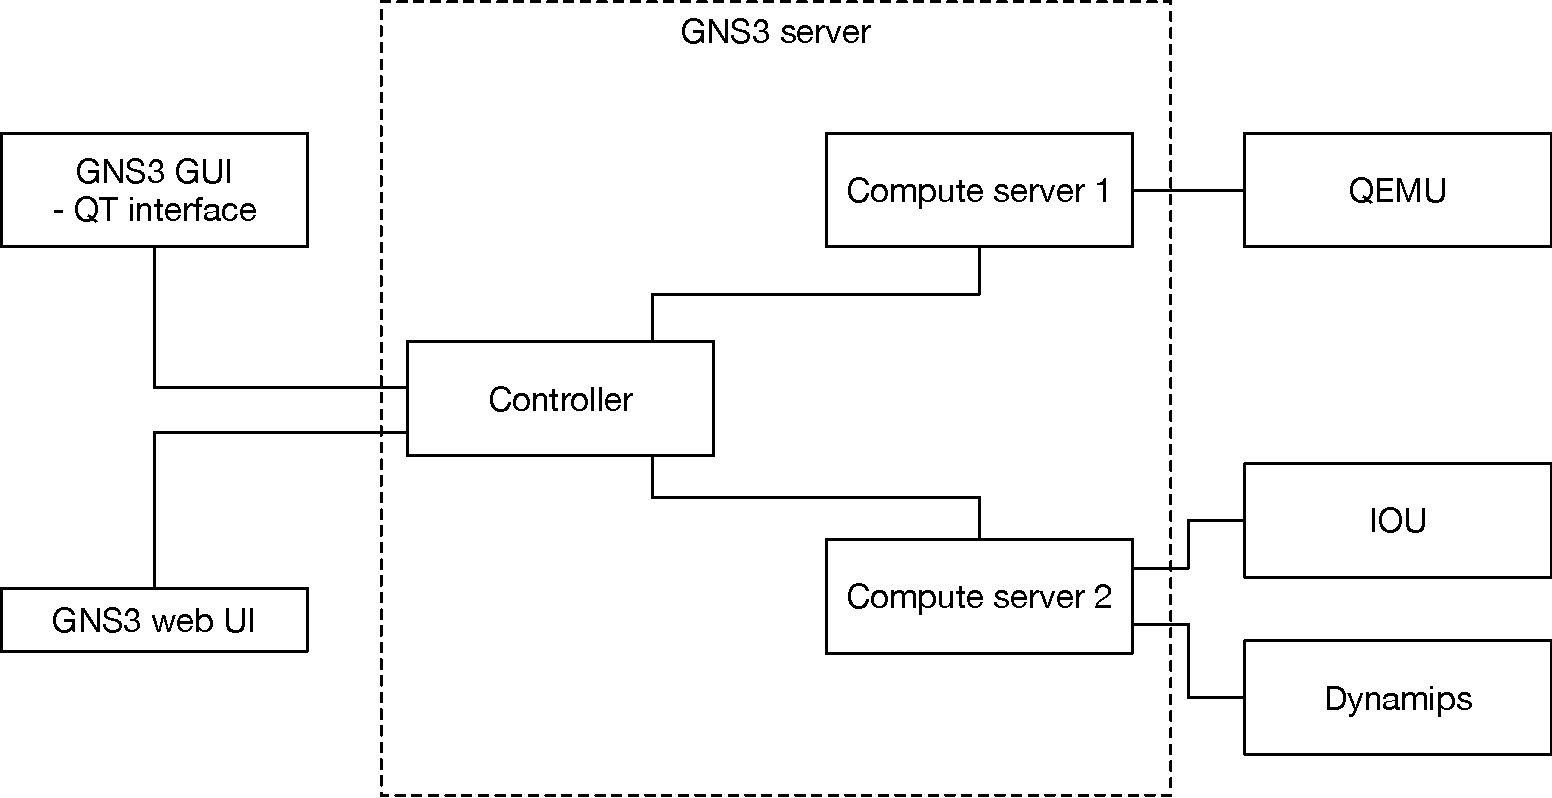
\includegraphics[width=0.8\textwidth]{gns3-docs-arch}
  \caption{The architecture of GNS3 (adapted from the official documentation)}
  \label{fig:gns3-docs-arch}
\end{figure}

% What follows is a description of what are those elements and what they do work internally.
% How they integrate with GNS3 or vice-versa, and also how they interact with each other, is described in~\ref{sec:gns3architecture}.

\begin{figure}
  \centering
  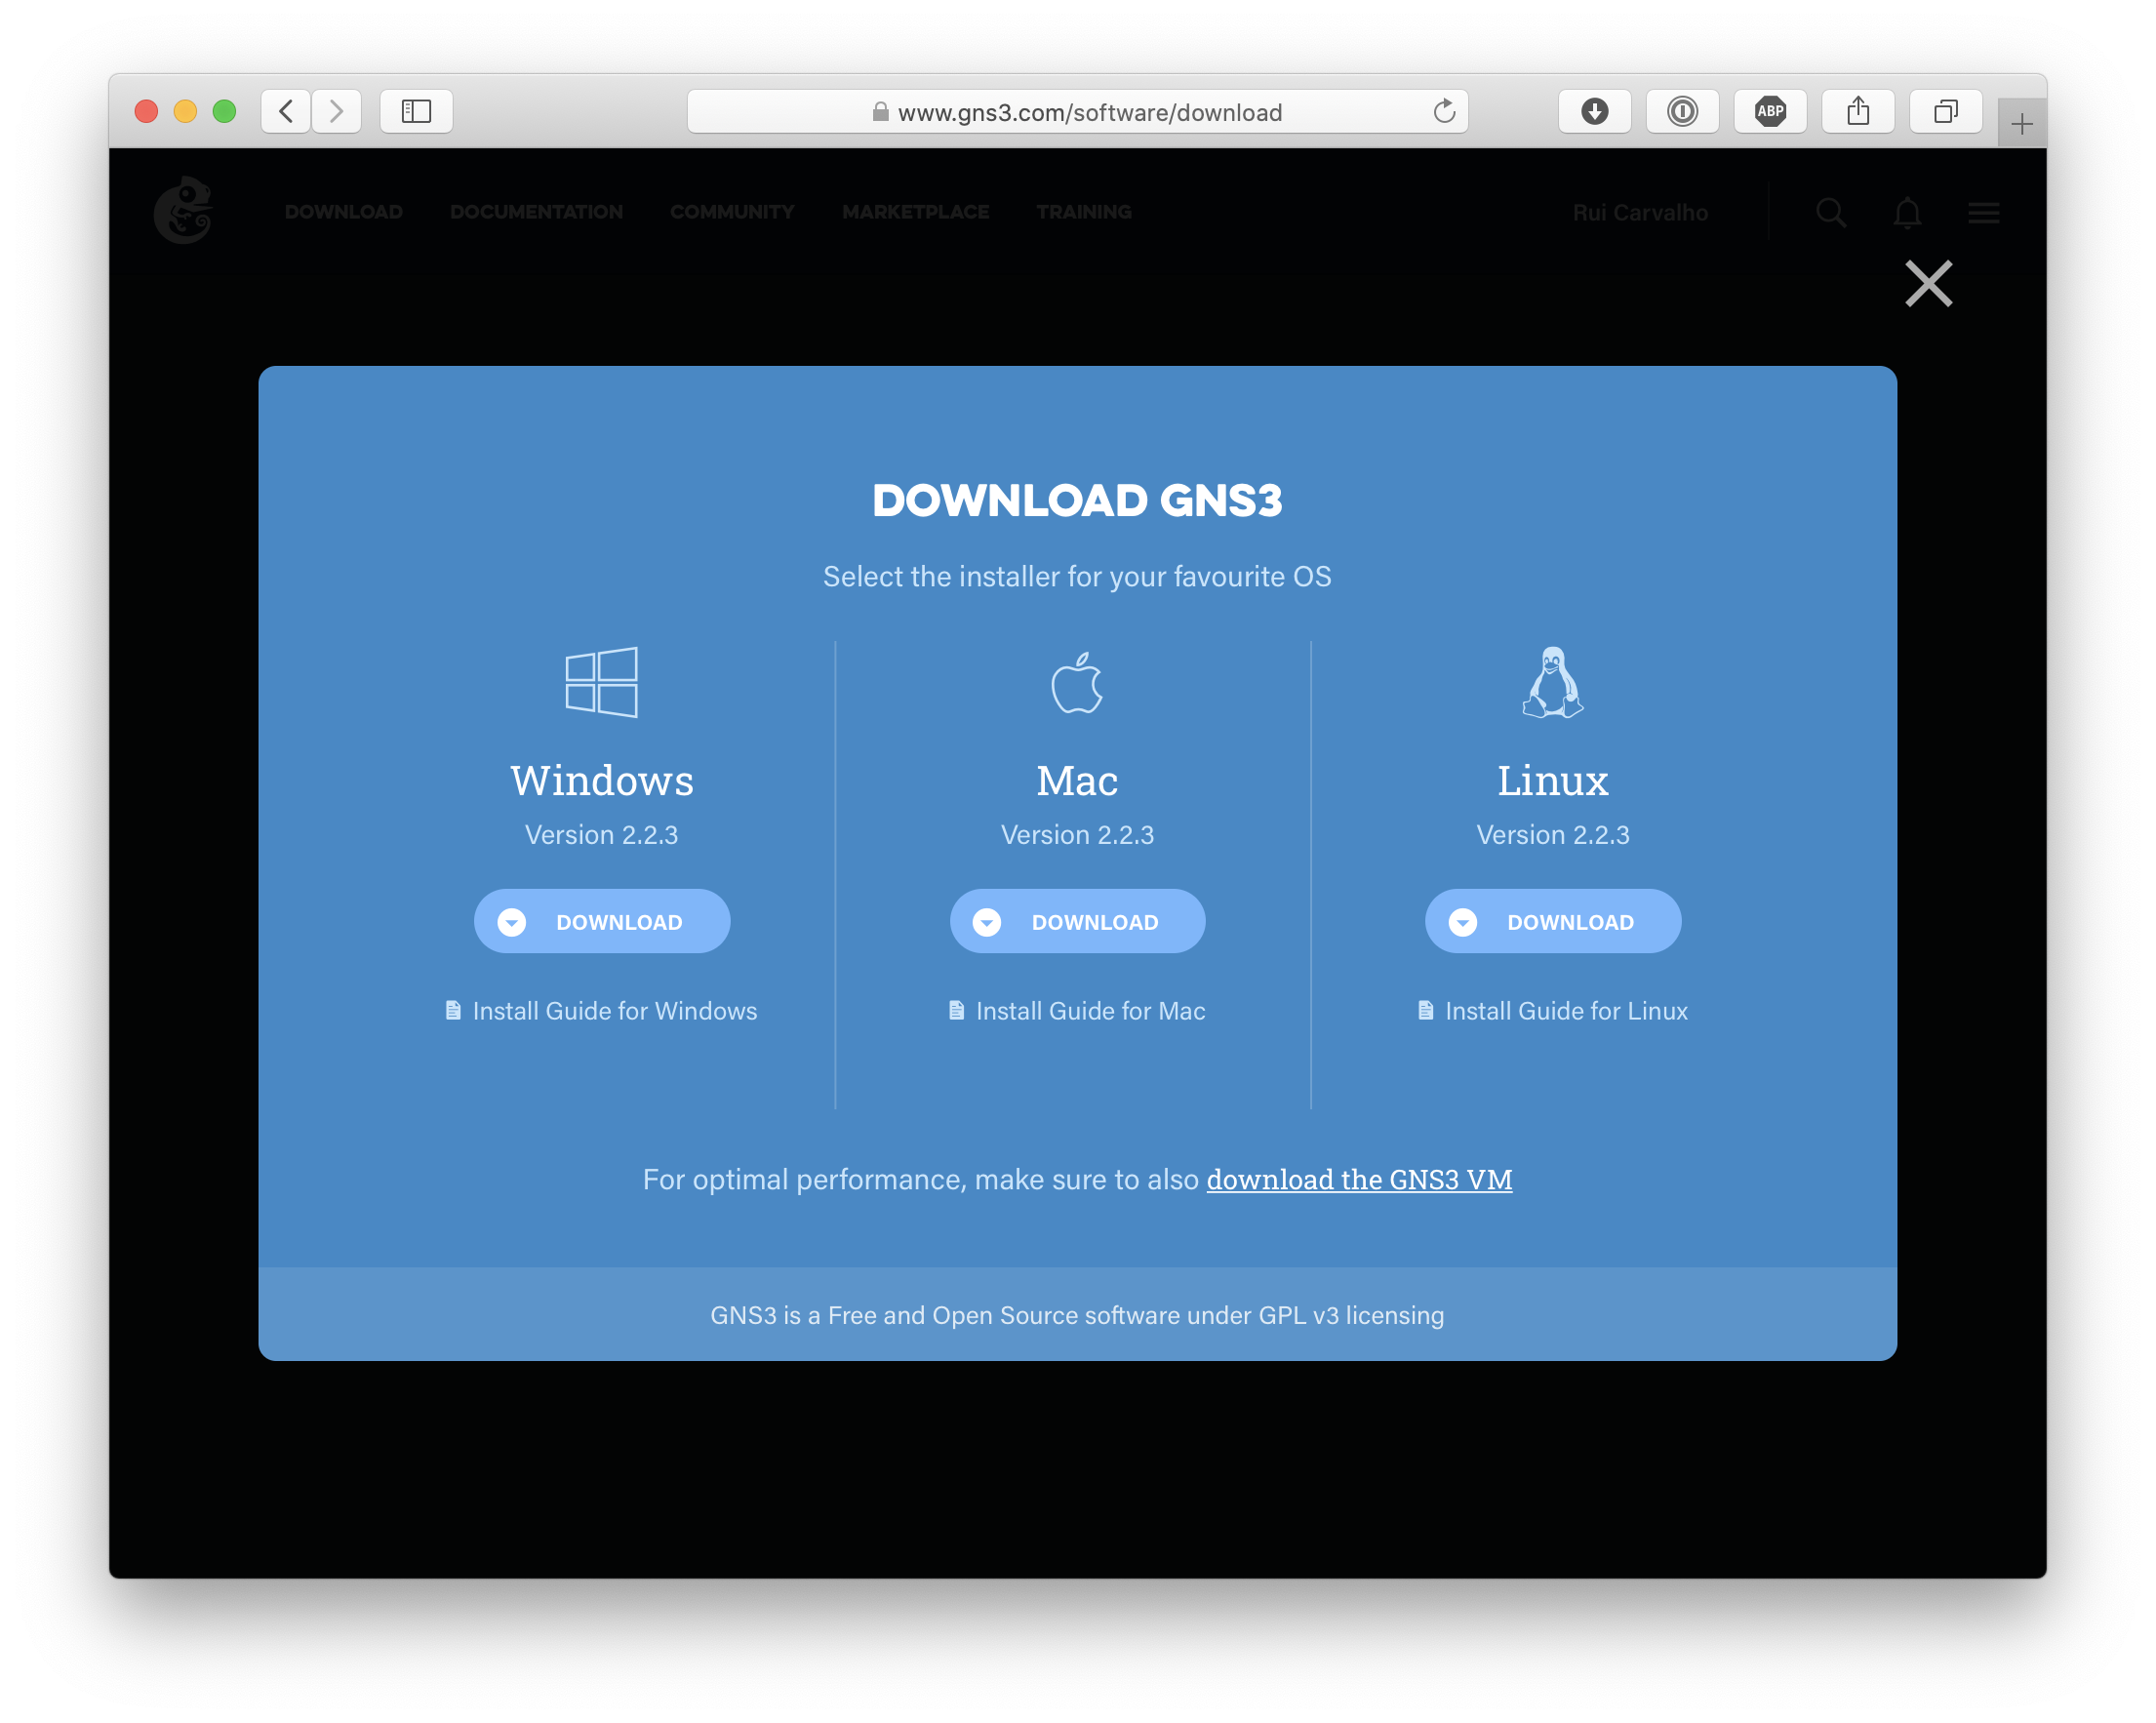
\includegraphics[width=0.8\textwidth]{download-gns3}
  \caption{The download screen on the official GNS3 website}
  \label{fig:download-gns3}
\end{figure}

When GNS3 is installed downloading one of its desktop distributions---available for Windows, macOS, and GNU/Linux, like the screen shot~\ref{fig:download-gns3} shows---, a user is installing multiple ``programs'' (or applications, whichever is the preferred denomination), implemented in disjunct codebases, and, given that they are \emph{free and open source} projects~\cite{gplv3}, hosted in GitHub, are easily accessible---and developers can enhance features and provide bugfixes.
Those are the essential building blocks of GNS3 and table~\ref{tab:gns3components} can serve a summary of what those pieces are.
It's worth noting that they are all under the GNS3 organization in GitHub\footnote{\url{https://github.com/gns3}}.

\begin{table}
  \centering
  \small
  \begin{tabulary}{0.8\textwidth}{lLL}
    \toprule
      \textbf{Part}  & \textbf{Role}                                                       & \textbf{Source code repository}\\
    \midrule
      GNS3 GUI       & A desktop application that runs on a graphical OS                   & \scriptsize\url{https://github.com/GNS3/gns3-gui}\\
      Dynamips       & A MIPS emulator, used by the \emph{backend} to run (old) IOS images & \scriptsize\url{https://github.com/GNS3/dynamips}\\
    \bottomrule
  \end{tabulary}
  \caption{%
    Intrinsic parts of GNS3, constituting separate and independent codebases
  }
  \label{tab:gns3components}
\end{table}


\subsection{GNS3 GUI}
\label{subsec:gns3gui}

Interaction between the end-user and GNS3 is usually---though, as will be clear, not necessarily---done in a graphical environment.
A GNS3 project, called a \emph{topology}, is constantly opened on one single window (per running instance of the application) and is graphically represented in the main section of the window.

Even though the GUI is not the authoritative source of truth for a topology (cf.~\ref{sec:gns3architecture}), it can be used as interface to all of GNS3's functionality: edit the topology itself (adding or removing nodes, changing links), performing actions on the nodes (like starting or stopping a host or router), or using helpers to launch consoles automatically connected via \texttt{telnet} or SSH.
In the section dedicated to the usage of GNS3~\ref{sec:gns3inaction}, it will be shown how this is done from a user's perspective.
Many GUI clients, on different hosts (e.g. laptops), can be editing the same topology at the same time. % TODO try to capture screenshots of this happening (use VMs)

\begin{figure}
  \centering
  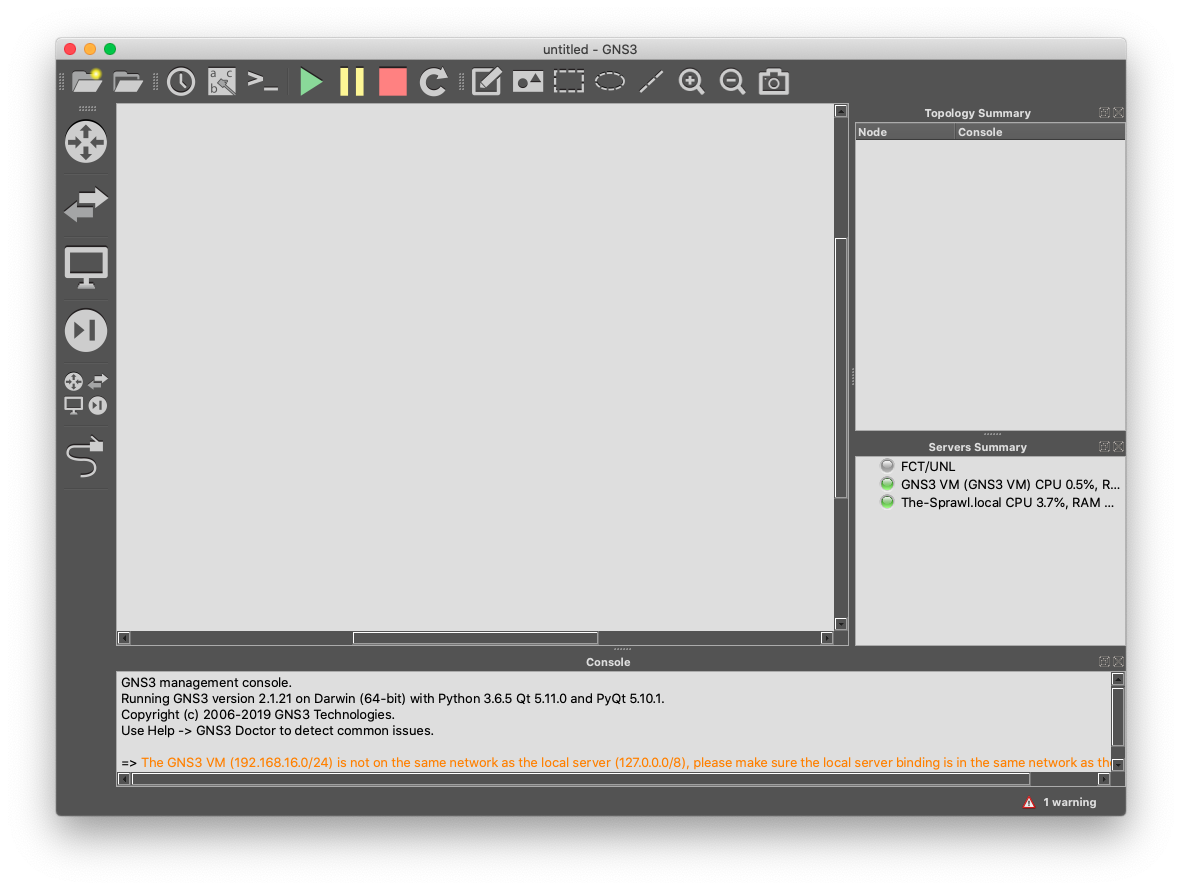
\includegraphics[width=0.8\textwidth]{gns3-empty-topology}
  \caption{An empty GNS3 topology shown in the GUI}
  \label{fig:gns3-empty-topology}
\end{figure}

\subsection{Dynamips}
\label{subsec:gns3dynamips}

The Dynamips emulator is a standalone program, written in C, that, usually, comes distributed together with the whole GNS3 package.
It is an emulator for a MIPS processor and was the original--single way to run the software of the Cisco nodes of the topologies created with GNS3.


\subsection{GNS3 server}
\label{subsec:gns3server}


\subsection{GNS3 VM}
\label{subsec:gns3vm}

% end of section gns3buildingblocks


\section{General architecture}
\label{sec:gns3architecture}

\begin{figure}
  \centering
  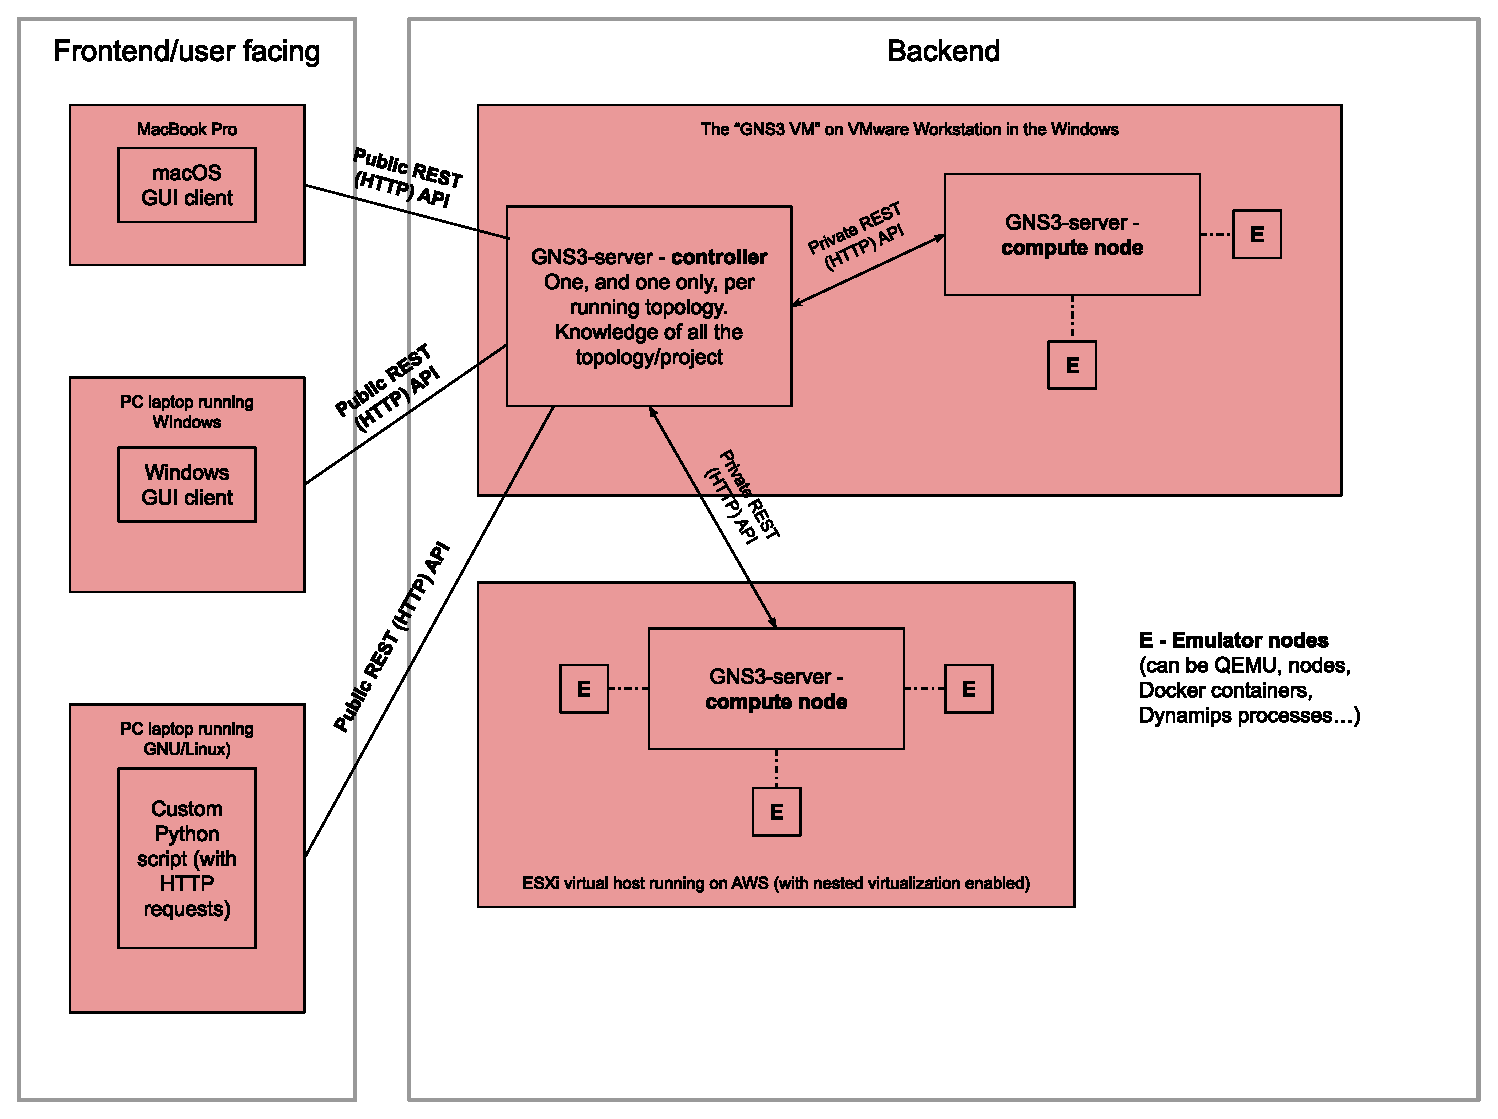
\includegraphics[width=1\textwidth]{gns3-running-arch}
  \caption{The GNS3 architecture}
  \label{fig:gns3-running-arch}
\end{figure}

In this section, an attempt is made to describe the different parts of GNS3 is to see what role they play in an execution of a topology (i.e. a project) and how they communicate with each other.
The diagram in figure~\ref{fig:gns3-running-arch} is based upon~\cite{ytgns3arch22}.
A central idea is the potentially distributed nature of the components, allowing for a complex topology with many nodes to be run across many hosts, dividing the computing power load across more than one host.
The precautions that must be taken to ensure a performance, and some caveats, will be explained in~\ref{sec:gns3inaction}. % TODO precautions taken?

The GNS3 server program, has two possible roles in a GNS3 session. % TODO define what's a "GNS3 session"
Those are: ``computes'' and the controller.
A GNS3 session only has one controller.
Any desktop installation of GNS3 comes with the server installed, able to run as the controller.
The GNS3 GUI will connect to the controller and allow for the user to ``open'' a topology on it.
The communication, as said, between any client (the GUI or any script) and the controller happens through HTTP requests following a REST approach. % TODO link acronyms et al to gls
The controller has knowledge of all the hosts running nodes of the topology.
Those nodes are run using ``computes'', which are processes of the GNS3 server whose responsibility is to expose a private REST API---\emph{not the same} as the one that the controller exposes and only to be used internally---to receive commands from the decision point (the controller) and locally interact with QEMU processes, Docker containers, Dynamips processes, or other emulation, container, or virtualization solution over which a node of the topology (an IOS Cisco router, a host, or a NAT node) is executed.

Therefore, on the diagram depicted in figure~\ref{fig:gns3-running-arch}, we see a topology running on distributed machines---these could be exclusively interconnected virtual machines on the same physical computer, without any loss of generality. % TODO put the background of the word of the same color that it has on the diagram
What matters is that they are running in hosts able to communicate with each other via IP and where GNS3 server is supported.
Each magenta rectangle is a separate host. % TODO check the color name
On the backend there are two hosts.
One of the hosts is the ``GNS3 VM'', running over VMware Workstation for Windows, and is ``playing'' both roles of the GNS3 server at the same time: it is the (single) controller for the running topology, which means that it loads the file describing the topology and has the receives the client's input, while knowing on which host should each topology node by run.
Then, it has a compute running alongside, to run two topology nodes.
These can be, for example, Cisco IOSv routers. % TODO how to spell IOSv. Somewhere we need to talk about this
On another host, which is a ESXi virtual machine (running on some infrastructure), \emph{with nested virtualization enabled}, the GNS3 server is also running, but there is no controller---all it does is ``blindly'' (at specific requests from the controller via the private REST API) perform, in the compute nodes, the necessary local interactions with the emulators. % TODO ESXi cite/link something
In the picture, there are three nodes running, which can be, for example, a Dynamips emulator for a <supported Dynamips Cisco router> and two hosts running on Docker. % TODO replce with a real model

% end of section gns3architecture

\section{GNS3 in action}
\label{sec:gns3inaction}

% end of section gns3inaction

\section{Performance and resources considerations}
\label{sec:gns3performance}

% end of section gns3performance

% end of chapter
 % Chapter 3
  % !TEX root = ../Thesis.tex
% !TEX spellcheck = en-US

\chapter{Kathará}
\label{ch:kathara}

Kathará~\cite{kathara} is a new implementation, created at the Roma Tre University using more modern technologies, of Netkit, a network emulator developed at the same institution years before.
It was made with the purpose of introducing functionalities of emulating SDN and NFV based networks, as well as leveraging the P4 language for programming forwarding-planes.
% Still, Kathará---as explicitly stated in the previously cited presentation article---is fully compatible with Netkit, having a similar interface and conceptual philosophy than its predecessor, in particular fully supporting topologies based in ``standard'' routing devices and generic hosts.

% Section "Functionality and studied usages"
\section{Functionality and studied usages}
\label{sec:katharafunctionality}

According to its developers, Kathará was built having in mind the creation of software framework, a computer network emulator, that allowed to prototype, develop over, and experiment with, not only traditional switched and routed networks, but also with four emerging concepts and technologies in the scope of (or related to) networking:
\begin{itemize}
	\item SDN
	\item NFV
	\item P4~\cite{p4programming} % TODO add to glossary
	\item Containers (and, in particular, Docker)
\end{itemize}

To build such a framework, the chosen starting point was an experimental tool called sdnetkit, which enhanced Netkit with OpenFlow enabled switches, still explicitly supporting ``traditional routers'' performing distributed routing protocols like OSPF~\cite{sdnkit}.
Kathará then evolved to be a fully backwards compatible tool with Netkit, using the same conceptual philosophy in terms of interfaces and emulated topology definition, with a substantially different implementation, and the capabilities of adding both P4 and OpenFlow enabled switches, and also nodes running the OS/framework ClockOS (proposed in~\cite{clockos}).

The high-level functional capabilities of Kathará explored in this work are the exactly the ones shared with the original Netkit---i.e. building and emulating topologies with traditional routers and switches and generic hosts.
However, as will be seen later, the implementation changes and overall modernization that Kathará brings can benefit any user.

Kathará's developers made the decision of considering a topology a set of nodes instantiated as Docker containers, communicating using Docker's low-level primitives

% end of section katharafunctionality


% Section "Functionality and studied usages"
\section{Architecture}
\label{sec:katharaarchitecture}

% end of section katharaarchitecture


% Section "Practical case study"
\section{Practical case study}
\label{sec:katharapracticalcasestudy}

% end of section katharapracticalcasestudy


% Section "Practical case study"
\section{Performance and resources considerations}
\label{sec:katharaperformance}

% end of section katharaperformance


% end of chapter
 % Chapter 4
  % !TEX root = ../Thesis.tex
% !TEX spellcheck = en-US

\chapter{Comparative analysis}
\label{ch:comparativeanalysis}

\section{Functionality}
\label{sec:comparativefunctionality}

\section{Performance and resource consumption}
\label{sec:comparativeperformance}

% end of chapter
 % Chapter 5
  % !TEX root = ../Thesis.tex
% !TEX spellcheck = en-US

\chapter{Conclusions and further work}
\label{ch:conclusions}

% \section{Section 1}
% \label{sec:relsec1}

% \section{Section 2}
% \label{sec:relsec2}

% end of chapter
 % Chapter 6

% This ensures that the subsequent sections are being included as root
% items in the bookmark structure of your PDF reader.
\bookmarksetup{startatroot}
\backmatter

  \begingroup
    \let\clearpage\relax
    \glsaddall
    \printglossary[type=\acronymtype]
    \newpage
    \printglossary
  \endgroup

  \printindex
  \printbibliography

\end{document}
